 
%
% SECTION: Run-through of the method
%
\section{Run-through of the method}
\begin{frame}
    \frametitle{Summary}
    \begin{columns}[t]
        \begin{column}{5cm}
            \tableofcontents[sections={1-3}, currentsection, hideothersubsections]
        \end{column}
        \begin{column}{5cm}
            \tableofcontents[sections={4-5}, currentsection, hideothersubsections]
        \end{column}
    \end{columns}
\end{frame}
\subsection{Method...}
\begin{frame}
    \frametitle{Title...}
    \framesubtitle{}
\end{frame}




\subsection{A method}
\begin{frame}
    \frametitle{Une méthode Structurée, Itérative et Qualitative}
    \framesubtitle{}
    \begin{columns}[t]
        \column{6.0cm}
        \begin{figure}
        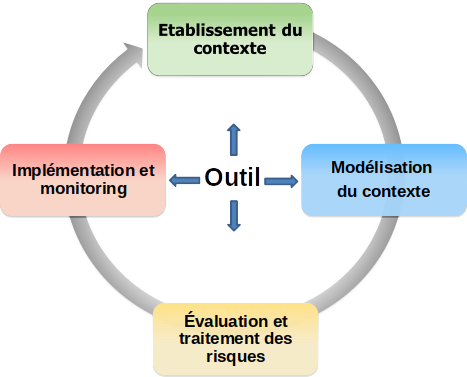
\includegraphics[width=6.0cm]{./images/MONARC-method-1.png}
        \end{figure}
        \column{6cm}
        \begin{itemize}
                \item Structurée: 1, 2, ..., n.
                \item Itérative: \textbf{Plan}, \textbf{Do}, \textbf{Check}, \textbf{Act}
                \item Qualitative: Impact/Conséquence, Menace, Vulnérabilité
        \end{itemize}
        \end{columns}
\end{frame}


\begin{frame}
    \frametitle{}
    \framesubtitle{Une gestion automatisée et simplifiée}
    \begin{center}
        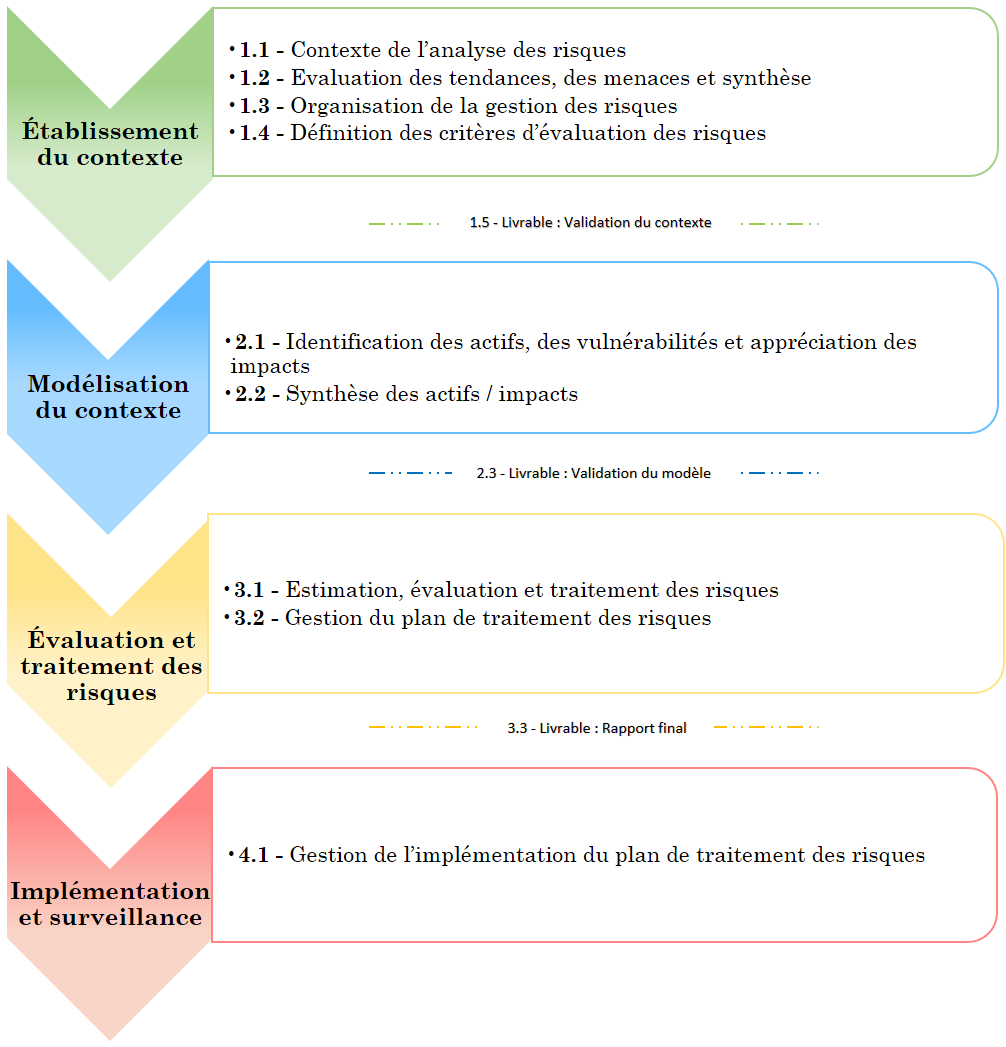
\includegraphics[scale=0.5]{./images/MONARC-method-2.png}
    \end{center}
\end{frame}


\begin{frame}
    \frametitle{Gestion de risques construite autour de la norme ISO/IEC 27005:2011}
    \framesubtitle{}
    \begin{block}{Risques de l’information}
        $$R = I \times M \times V$$
        \begin{itemize}
            \item Impact on CID;
            \item secondary assets.
        \end{itemize}
    \end{block}


    \begin{block}{Risques opérationnels}
        $$R = I \times P$$
        \begin{itemize}
            \item Impact on ROLFP. Brut/Net;
            \item primary assets
        \end{itemize}
    \end{block}
\end{frame}


\begin{frame}
    \frametitle{Optimisations}
    \framesubtitle{}
    \begin{block}{Une méthode optimisée}
    Héritage, portée des objets, modèles, livrables.
    \end{block}
\end{frame}
